Table~\ref{tab:main} gives mean test Spearman and mean design\_hit over five seeds for the eight main tasks at $N=1000$; per-seed standard deviations of both endpoints are in Table~\ref{tab:sd}, and Fig.~\ref{fig:K} plots both endpoints against $K$. Comparisons are paired over seeds. Paired $t$-tests come from \texttt{rh compare} (files \texttt{results/tables/compare\_main\_*.csv}); the Wilcoxon tests, rank correlations and tests against the exact chance rate come from \texttt{analysis/hyp.py} (\texttt{results/hypotheses.txt}). With $n=5$ and no correction for multiple comparisons, all $p$-values are indicative only. All statements below are about simulated NK landscapes at two $(L,A)$ settings in which $L$ and $A$ change together.

\begin{table*}[t]\centering\caption{Simulated NK landscapes, $N=1000$ training variants, 5000 test variants, mean over 5 seeds. Left: held-out Spearman; right: design\_hit (fraction of the 10 proposed single mutants of the best measured sequence that beat it). Chance: mean fraction of \emph{all} single mutants of the parent that beat it, i.e.\ the exact expected hit rate of random proposals, of which the Random column is a noisy 10-proposal estimate. Bold: best of the four learned systems (Random excluded; ties in bold).}\label{tab:main}\begin{tabular}{lrrrrr|rrrrrr}
\toprule
 & \multicolumn{5}{c|}{Spearman} & \multicolumn{6}{c}{design\_hit}\\
Task & Add. & Pair. & CNN & MLP & Rand. & Add. & Pair. & CNN & MLP & Rand. & Chance\\
\midrule
L15\_A4\_K0 & \textbf{1.000} & \textbf{1.000} & 0.999 & 0.999 & 0.003 & \textbf{0.98} & \textbf{0.98} & 0.92 & 0.94 & 0.32 & 0.258\\
L15\_A4\_K1 & 0.596 & \textbf{0.998} & 0.746 & 0.815 & 0.002 & 0.38 & \textbf{0.90} & 0.40 & 0.52 & 0.28 & 0.213\\
L15\_A4\_K2 & 0.310 & \textbf{0.508} & 0.384 & 0.383 & -0.000 & 0.10 & 0.18 & 0.18 & \textbf{0.22} & 0.14 & 0.102\\
L15\_A4\_K4 & 0.079 & \textbf{0.080} & 0.065 & 0.063 & -0.001 & \textbf{0.10} & 0.08 & 0.08 & 0.08 & 0.06 & 0.067\\
\midrule
L20\_A20\_K0 & \textbf{1.000} & 0.995 & 0.965 & 0.994 & -0.007 & \textbf{1.00} & \textbf{1.00} & \textbf{1.00} & \textbf{1.00} & 0.38 & 0.263\\
L20\_A20\_K1 & 0.110 & \textbf{0.138} & 0.077 & 0.090 & 0.009 & 0.34 & \textbf{0.38} & 0.30 & 0.32 & 0.24 & 0.233\\
L20\_A20\_K2 & 0.021 & \textbf{0.025} & 0.013 & 0.020 & 0.007 & \textbf{0.34} & 0.30 & 0.14 & 0.16 & 0.14 & 0.185\\
L20\_A20\_K4 & \textbf{0.014} & \textbf{0.014} & 0.006 & 0.013 & 0.008 & \textbf{0.18} & 0.14 & 0.04 & 0.16 & 0.08 & 0.115\\
\bottomrule
\end{tabular}
\end{table*}

\begin{figure*}[t]\centering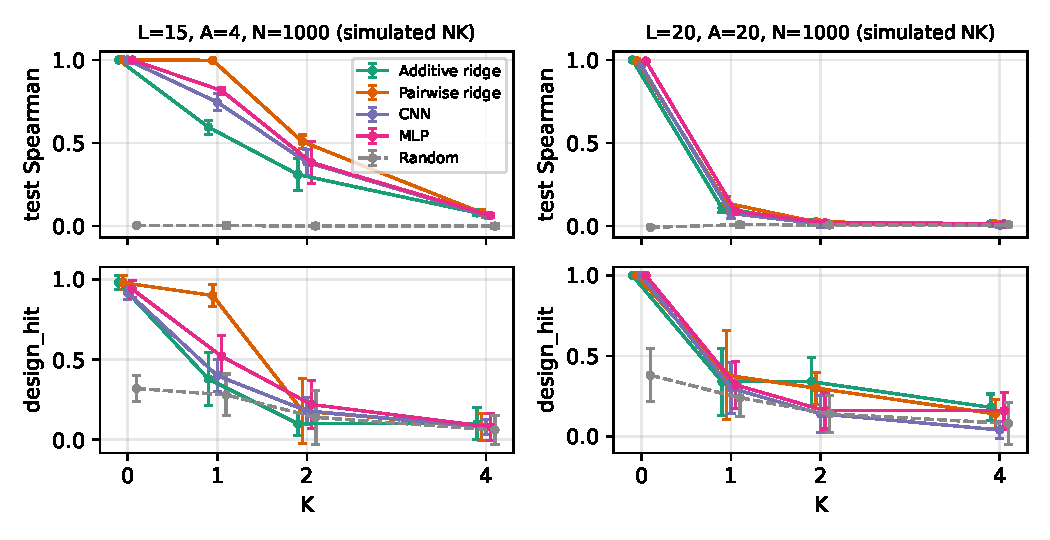
\includegraphics[width=\textwidth]{generated/fig_vs_K.pdf}\caption{Spearman (top) and design\_hit (bottom) versus $K$ for the two $(L,A)$ settings, $N=1000$; mean $\pm$ SD over 5 seeds. Everything is simulated.}\label{fig:K}\end{figure*}

\begin{table*}[t]\centering\caption{Standard deviation over the 5 seeds of test Spearman and of design\_hit (same cells as Table~\ref{tab:main}).}\label{tab:sd}\begin{tabular}{lrrrr|rrrrr}
\toprule
 & \multicolumn{4}{c|}{SD of Spearman} & \multicolumn{5}{c}{SD of design\_hit}\\
Task & Add. & Pair. & CNN & MLP & Add. & Pair. & CNN & MLP & Rand.\\
\midrule
L15\_A4\_K0 & 0.000 & 0.000 & 0.000 & 0.000 & 0.04 & 0.04 & 0.04 & 0.05 & 0.08\\
L15\_A4\_K1 & 0.042 & 0.002 & 0.052 & 0.020 & 0.16 & 0.07 & 0.10 & 0.13 & 0.13\\
L15\_A4\_K2 & 0.096 & 0.040 & 0.079 & 0.126 & 0.07 & 0.20 & 0.08 & 0.15 & 0.17\\
L15\_A4\_K4 & 0.017 & 0.019 & 0.011 & 0.011 & 0.10 & 0.08 & 0.04 & 0.08 & 0.09\\
\midrule
L20\_A20\_K0 & 0.000 & 0.000 & 0.005 & 0.002 & 0.00 & 0.00 & 0.00 & 0.00 & 0.16\\
L20\_A20\_K1 & 0.029 & 0.038 & 0.032 & 0.022 & 0.21 & 0.28 & 0.16 & 0.15 & 0.11\\
L20\_A20\_K2 & 0.016 & 0.015 & 0.020 & 0.017 & 0.15 & 0.10 & 0.11 & 0.11 & 0.11\\
L20\_A20\_K4 & 0.010 & 0.008 & 0.011 & 0.011 & 0.08 & 0.09 & 0.05 & 0.11 & 0.13\\
\bottomrule
\end{tabular}
\end{table*}

\paragraph{H1 (additive models absorb an additive landscape): supported.} At $K=0$ additive ridge reaches Spearman $\rhval{main/additive-ridge/l15_a4_k0/spearman/mean:3}$ at $(15,4)$ and $\rhval{main/additive-ridge/l20_a20_k0/spearman/mean:3}$ at $(20,20)$ (threshold $0.95$). The MLP reaches $\rhval{main/mlp/l20_a20_k0/spearman/mean:3}$ at L20\_A20\_K0, while the CNN is lower at $\rhval{main/cnn/l20_a20_k0/spearman/mean:3}$ (Table~\ref{tab:main}); at $K=0$ neither network improves on additive ridge. This is a sanity check on the simulator and the pipeline, not a finding.

\paragraph{H2 (epistasis hurts the additive model; pairs recover K=1): supported, but weakly at $(20,20)$.} Additive Spearman falls from $\rhval{main/additive-ridge/l15_a4_k0/spearman/mean:3}$ to $\rhval{main/additive-ridge/l15_a4_k1/spearman/mean:3}$, $\rhval{main/additive-ridge/l15_a4_k2/spearman/mean:3}$, $\rhval{main/additive-ridge/l15_a4_k4/spearman/mean:3}$ for $K=0,1,2,4$ at $(15,4)$, and from $\rhval{main/additive-ridge/l20_a20_k0/spearman/mean:3}$ to $\rhval{main/additive-ridge/l20_a20_k1/spearman/mean:3}$, $\rhval{main/additive-ridge/l20_a20_k2/spearman/mean:3}$, $\rhval{main/additive-ridge/l20_a20_k4/spearman/mean:3}$ at $(20,20)$. Pairwise ridge beats additive ridge at $K=1$ in all five seeds on both tasks (so the one-sided Wilcoxon test of \texttt{analysis/hyp.py} takes its smallest attainable $p$-value with five seeds, $1/32$). At $K=1$ every contribution $T_i$ is a function of two sites, so the model class contains the truth: at (15,4) the pairwise model reaches $\rhval{main/pairwise-ridge/l15_a4_k1/spearman/mean:3}$ versus $\rhval{main/additive-ridge/l15_a4_k1/spearman/mean:3}$. At (20,20) the gain is only $\rhval{main/pairwise-ridge/l20_a20_k1/spearman/mean:3}$ versus $\rhval{main/additive-ridge/l20_a20_k1/spearman/mean:3}$. A plausible reason is that $76{,}000$ pair coefficients must be estimated from 1000 sequences; this is consistent with, but not isolated by, the $N$ sweep and the oracle-graph ablation of Sec.~\ref{sec:ablations}.

\paragraph{H3 (small networks do not beat pairwise ridge at this scale): supported at $N=1000$.} Neither the CNN nor the MLP exceeds pairwise ridge in mean Spearman in any of the six cells with $K\ge1$ (Table~\ref{tab:main}). The networks have higher means than additive ridge on L15\_A4\_K1 and L15\_A4\_K2 ($\rhval{main/cnn/l15_a4_k1/spearman/mean:3}$/$\rhval{main/mlp/l15_a4_k1/spearman/mean:3}$ and $\rhval{main/cnn/l15_a4_k2/spearman/mean:3}$/$\rhval{main/mlp/l15_a4_k2/spearman/mean:3}$ versus $\rhval{main/additive-ridge/l15_a4_k1/spearman/mean:3}$ and $\rhval{main/additive-ridge/l15_a4_k2/spearman/mean:3}$ for CNN/MLP/Additive; at $K=2$ the differences are within the seed SDs of Table~\ref{tab:sd}), i.e.\ at $K=1$ they absorb some non-additivity, but less than the model that has pair features built in. At $(20,20)$ their means are at or below additive ridge. The CNN's locality prior may be a poor match for the random-neighbour structure of these landscapes; we did not test this, nor other architectures, so this is not a statement about CNNs in general.

\paragraph{H4 (design success tracks prediction): registered criterion met, evidence weak.} The registered test is that, across the 40 (task, seed) units, the Spearman correlation between the Pairwise$-$Additive gain in test Spearman and the gain in design\_hit is positive. It is positive (\texttt{results/hypotheses.txt}, Fig.~\ref{fig:delta}). Its nominal $p$-value treats the 40 units as independent, which they are not (five seeds in each of eight tasks), and the association is carried by one cell, L15\_A4\_K1, where pairwise ridge reaches design\_hit $\rhval{main/pairwise-ridge/l15_a4_k1/design_hit/mean:2}$ versus $\rhval{main/additive-ridge/l15_a4_k1/design_hit/mean:2}$ for additive ridge (Table~\ref{tab:h4}): without that cell the correlation is smaller and not nominally significant, and over the eight task means it is not nominally significant either (\texttt{results/hypotheses.txt}). On L15\_A4\_K2, a Spearman gain from $\rhval{main/additive-ridge/l15_a4_k2/spearman/mean:3}$ to $\rhval{main/pairwise-ridge/l15_a4_k2/spearman/mean:3}$ comes with a design\_hit change from $\rhval{main/additive-ridge/l15_a4_k2/design_hit/mean:2}$ to $\rhval{main/pairwise-ridge/l15_a4_k2/design_hit/mean:2}$ only (paired $t$-test $p=\rhval{cmp/main/pairwise-ridge/l15_a4_k2/design_hit/paired_p:2}$, Table~\ref{tab:h4}), within the seed spread of Table~\ref{tab:sd}. So prediction gains translated into a clear design gain in one cell only.

The second part of the registered test holds for the means: at $K\le1$ every learned model's mean design\_hit exceeds Random's and the exact chance rate (Table~\ref{tab:main}). The margin is large at $K=0$ and for pairwise ridge at L15\_A4\_K1. Elsewhere it is not: at L20\_A20\_K1 all four learned models ($\rhval{main/cnn/l20_a20_k1/design_hit/mean:2}$ to $\rhval{main/pairwise-ridge/l20_a20_k1/design_hit/mean:2}$ versus $\rhval{main/random/l20_a20_k1/design_hit/mean:2}$ for Random and $\rhval{main/random/l20_a20_k1/frac_mutants_better/mean:3}$ for chance) are within their seed SDs ($\rhval{main/mlp/l20_a20_k1/design_hit/std:2}$ to $\rhval{main/pairwise-ridge/l20_a20_k1/design_hit/std:2}$), and at L15\_A4\_K1 the additive, CNN and MLP margins over the Random system are not distinguishable from noise in paired $t$-tests (\texttt{rh compare}), although the CNN and MLP are nominally above the exact chance rate there (\texttt{results/hypotheses.txt}).

At $K\ge2$ no learned model's design\_hit differs from Random's in paired $t$-tests (\texttt{rh compare} with Random as the reference, \texttt{results/tables/compare\_main\_design\_hit\_ref\_random.csv}; four tasks, four models; the unpaired Welch test in the same output is nominally at the conventional threshold for additive and pairwise ridge at L20\_A20\_K2, $p=\rhval{cmp/main/random/l20_a20_k2/design_hit/welch_p:2}$ for additive ridge). One pattern in the means is left unexplained: at L20\_A20\_K2 and L20\_A20\_K4 additive ridge has design\_hit $\rhval{main/additive-ridge/l20_a20_k2/design_hit/mean:2}$ and $\rhval{main/additive-ridge/l20_a20_k4/design_hit/mean:2}$, against $\rhval{main/random/l20_a20_k2/design_hit/mean:2}$ and $\rhval{main/random/l20_a20_k4/design_hit/mean:2}$ for Random and $\rhval{main/random/l20_a20_k2/frac_mutants_better/mean:3}$ and $\rhval{main/random/l20_a20_k4/frac_mutants_better/mean:3}$ for chance, while its Spearman on random test sequences is low ($\rhval{main/additive-ridge/l20_a20_k2/spearman/mean:3}$, $\rhval{main/additive-ridge/l20_a20_k4/spearman/mean:3}$; Random $\rhval{main/random/l20_a20_k2/spearman/mean:3}$, $\rhval{main/random/l20_a20_k4/spearman/mean:3}$). With five seeds of 10 proposals these margins are not distinguishable from noise (paired $t$-test $p=\rhval{cmp/main/random/l20_a20_k2/design_hit/paired_p:2}$ and $\rhval{cmp/main/random/l20_a20_k4/design_hit/paired_p:2}$ against Random, Table~\ref{tab:h4}; the tests against the exact chance rate in \texttt{results/hypotheses.txt} are not nominally significant either), so we draw no conclusion from them. Whether a model can rank the single mutants of one parent while its Spearman on random, far-apart sequences is near zero would need more seeds and larger proposal batches to test.

\begin{table}[t]\centering\caption{H4 details: mean paired difference in design\_hit over 5 seeds (reference minus the other system) with a two-sided paired $t$-test, from \texttt{rh compare} with additive ridge as the reference. $p$-values are nominal and uncorrected. The rank correlations of the registered test and the tests against the exact chance rate are in \texttt{results/hypotheses.txt}.}\label{tab:h4}
\begin{tabular}{lrr}
\toprule
Quantity & Value & $p$\\
\midrule
Add.$-$Pair. hit, L15\_A4\_K1 & \rhval{cmp/main/pairwise-ridge/l15_a4_k1/design_hit/delta:2} & \rhval{cmp/main/pairwise-ridge/l15_a4_k1/design_hit/paired_p:3}\\
Add.$-$Pair. hit, L15\_A4\_K2 & \rhval{cmp/main/pairwise-ridge/l15_a4_k2/design_hit/delta:2} & \rhval{cmp/main/pairwise-ridge/l15_a4_k2/design_hit/paired_p:2}\\
Add.$-$Pair. hit, L20\_A20\_K1 & \rhval{cmp/main/pairwise-ridge/l20_a20_k1/design_hit/delta:2} & \rhval{cmp/main/pairwise-ridge/l20_a20_k1/design_hit/paired_p:2}\\
\midrule
Add.$-$Rand. hit, L20\_A20\_K2 & \rhval{cmp/main/random/l20_a20_k2/design_hit/delta:2} & \rhval{cmp/main/random/l20_a20_k2/design_hit/paired_p:2}\\
Add.$-$Rand. hit, L20\_A20\_K4 & \rhval{cmp/main/random/l20_a20_k4/design_hit/delta:2} & \rhval{cmp/main/random/l20_a20_k4/design_hit/paired_p:2}\\
\bottomrule
\end{tabular}\end{table}

\begin{figure}[t]\centering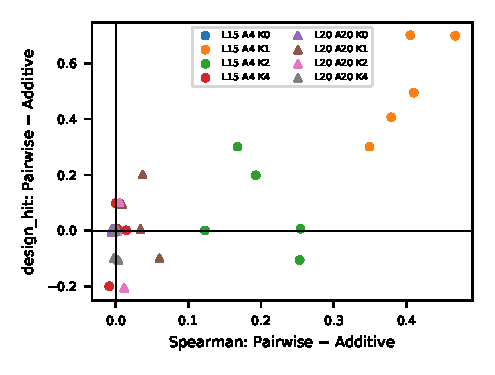
\includegraphics[width=0.85\columnwidth]{generated/fig_delta.pdf}\caption{Per (task, seed): gain of Pairwise over Additive in Spearman (x) versus in design\_hit (y; small vertical jitter added for display). Circles: $L=15,A=4$; triangles: $L=20,A=20$.}\label{fig:delta}\end{figure}

\paragraph{Where every model fails.} At $K=4$ for both settings and at $(20,20)$ with $K\ge2$, all four systems have mean Spearman of at most $\rhval{main/pairwise-ridge/l15_a4_k4/spearman/mean:3}$ and, for $(20,20)$, at most $\rhval{main/pairwise-ridge/l20_a20_k2/spearman/mean:3}$ (Table~\ref{tab:main}); differences between system means there are comparable to or smaller than the seed SDs (Table~\ref{tab:sd}), and on L20\_A20\_K4 all learned means ($\le\rhval{main/pairwise-ridge/l20_a20_k4/spearman/mean:3}$) are close to Random's ($\rhval{main/random/l20_a20_k4/spearman/mean:3}$). The data do not say whether more data would help in these regimes; the $N$ sweep only covers L15\_A4\_K2 and L20\_A20\_K1. Also, pairwise ridge is not the best system at $K=0$ at $(20,20)$ ($\rhval{main/pairwise-ridge/l20_a20_k0/spearman/mean:3}$ versus $\rhval{main/additive-ridge/l20_a20_k0/spearman/mean:3}$), which may be a small cost of fitting uninformative pair features: the oracle-graph variant, which has no pair features at $K=0$, reaches $\rhval{abl_pair/pairwise-ridge-oracle-graph/l20_a20_k0/spearman/mean:3}$ (Table~\ref{tab:abl}).
